\documentclass[conference]{IEEEtran}
\IEEEoverridecommandlockouts

\usepackage{cite}
\usepackage{amsmath,amssymb,amsfonts}
\usepackage{algorithmic}
\usepackage{graphicx}
\usepackage{textcomp}
\usepackage{xcolor}
\usepackage{booktabs}
\usepackage{tikz}
\usepackage{url}
\usetikzlibrary{arrows.meta,positioning,shapes.geometric}
\usetikzlibrary{calc,fit,backgrounds}

\begin{document}

\title{Group 3: Improving LLM Inference through Pairwise Ranking Scheduler and Median-Based Length Predictor}

\author{
\IEEEauthorblockN{Mohammed Sirajuddin, Anmol Saluja, Chandra Venigalla, Daisy Clavijo, Sravan Bhamidipati}
\IEEEauthorblockA{
Fairleigh Dickinson University, Vancouver, Canada
}
}

\maketitle

\begin{abstract}
Large language model serving systems usually just handle requests in the order they arrive — first-come-first-served. That's a problem because short requests get stuck behind long ones, since generation time depends mostly on output length, and you don't know how long the output will be until it's actually being decoded. Some prior work tried to approximate shortest-job-first scheduling by predicting output length with a separate model, but here's the thing: a single generation is a noisy training signal. The same prompt can produce wildly different lengths across runs — it's a heavy-tailed distribution. So pointwise regression targets don't really line up with what the scheduler actually needs, which is just the relative ordering of requests.

This report introduces a length-aware scheduler that uses robust median supervision — we call it ProD-M — combined with a pairwise learning-to-rank predictor inspired by PARS, plus some priority-aware starvation prevention. We sample Llama-3.2-3B three times per prompt, take the median output length as the label, train a lightweight MLP on the served model's own hidden states, and train a BERT-based pairwise ranker with margin ranking loss on median-labelled pairs. On a mixed workload of 1,000 prompts covering math, code, chat, and long-context tasks, our scheduler cuts average end-to-end latency by 42.9\% compared to FCFS and by 5.8\% compared to a pointwise learning-to-rank baseline. Throughput stays the same, and we hold the lowest latency at every arrival rate from 5 to 60 requests per second. The pairwise ranker orders the workload with a Kendall's Tau of about 0.93. We also quantify the tail-latency trade-off that comes with any SJF-style approach.
\end{abstract}

\section{Introduction}
Large language models power things like conversational assistants, code generators, and retrieval-augmented apps that need to handle thousands of simultaneous requests with low latency. The thing is, decoding is autoregressive — so how long a request takes depends almost entirely on how many output tokens it produces. And that number varies wildly. A simple factual query might finish in a dozen tokens. A competition math problem or code generation task? That can run into the thousands \cite{fu2024efficient,tao2025pars}.

Classical scheduling theory says shortest-job-first minimizes mean waiting time. That much is settled. But there's a catch — SJF needs job durations, and you can't know how long a generation will take before it's done.
So a lot of recent work tries to predict output length ahead of time. Some approaches ask the LLM to estimate its own response length \cite{zheng2023response}. Others train auxiliary classifiers or regressors on the prompt text \cite{jin2023s3,qiu2024ssjf}. Still others reuse the served model's internal representations \cite{shahout2025trail,xie2026egtp}. Two problems keep coming up though.

First, most methods treat output length as a fixed number. But if you generate the same prompt multiple times with the same settings, you get a heavy-tailed distribution of lengths. So a single sampled label introduces a lot of noise into training \cite{wang2026prodm}. Second, a scheduler doesn't actually need precise lengths. It needs the right ordering of requests. Pointwise regression optimizes for the wrong thing here.
Listwise ranking does better than regression \cite{fu2024efficient}. And pairwise ranking with margin loss plus filtering of near-tie pairs — that's been shown to focus training on the comparisons that actually matter for scheduling \cite{tao2025pars}.

This work, conducted as the CSCI 6806 graduate cap-stone, implements and evaluates a scheduler that combinesboth remedies. Following the robust-supervision perspectiveof ProD-M \cite{wang2026prodm}, we sample the served model r=3 times per prompt and use the median output length as the training label, which is the Bayes-optimal point target under mean absolute error and is far less sensitive to occasional very long generations than a single sample. Following PARS \cite{tao2025pars}, we train a BERT-based pairwise ranker with margin ranking loss on median-labelled prompt pairs, discarding pairs whose relative length difference falls inside the model's natural sampling variability. The resulting scores drive an SJF-style scheduler
with three priority classes and a starvation-prevention rule, and we compare it against FCFS and against the pointwise learning-to-rank (LTR) baseline of the main reference paper \cite{fu2024efficient} on a mixed workload of math, coding, chat, and long-
context prompts served by Llama-3.2-3B-Instruct \cite{dubey2024llama3}.

A ranker trained with noisy and single-sample labels can still get two prompts right if the noise is cancelled out, but this is of course not guaranteed and the errors will add up if a sampled length is very different from the length that is typically generated by a particular prompt. On the other hand, a strong median label is only useful to a scheduler if it is consumed with an objective that is actually of the sort that scheduling cares about, which is the relative ordering of requests, not an absolute length value. This work connects both contributions by training the pairwise ranker directly on the median-based labels, and by removing prompt pairs with length differences of the prompt's label that happen to fall within the model's sampling variance, to the detriment of increased offline computation required to produce the multiple samples per prompt that are needed to label.

This work has the following contributions:

\begin{itemize}
\item An end-to-end open-source pipeline for producing strong robust products. Trains length labels from a live LLM to provide median-supervised labels. Both a pointwise LTR baseline and a pairwise PARS-style ranker. Identifies three scheduling policies and measures them using identical conditions;

\item A comparison of memory and performance based on 1,000 mixed domain prompts is empirical. Shows a 42.9\% improvement in average latency compared to FCFS and 5.8\% compared with the pointwise LTR baseline at equal throughput, policy lowest at all arrivals sweep load and get a rate of 5--60 req/s;

\item A predictor study was performed on the same workload and demonstrated that: pairwise ranking over median labels orders requests with a Kendall's Tau of ~0.93 (very close to 1) and almost perfect Pearson's correlation were obtained. It's the same as pointwise length regression, except for NDCG. The mean absolute error for the labels is 46 tokens; and

\item An honest description of the mean-tail trade-off of SJF-style policies, in which p95 latency regresses while mean latency improves, along with an analysis, to the extent that priority boosting and starvation control bound this effect.
\end{itemize}

The remainder of this report is organised as follows.
Section~\ref{sec:background} provides the technical background: the two-phase
The statistics of prompt-conditioned output is called inference pipeline. In addition to length, we use learning-to-rank formulations and our system architecture. Section~\ref{sec:related-work} looks at the related work, categorized by approach family. Section~\ref{sec:methodology} details the methodology, platform, hyperparameters that allow to replicate all the outcomes. Section~\ref{sec:evaluation} presents the evaluation over various quality of predictors, training dynamics refers to the scheduler comparison, tail-latency behaviour, load etc.sensitivity, and cost. Section~\ref{sec:discussion} is an analysis of the results.Their limitations are explored and then Section~\ref{sec:conclusion} concludes.

\section{Background}
\label{sec:background}
This segment presents the technical basics needed to understand the design of the system: the dual-phase process of LLM inference and the point where HOL blocking happens, the information related to the output length dependent on the given prompt, the learning-to-rank methods and the design of the system.

\subsection{Process of LLM Serving Pipeline and HOL Blocking LLM inference}\label{sec:hol-blocking}

 In the first stage, the whole prompt is processed at once which leads to filling the key-value (KV) cache; this stage is dependent on computing. The second stage implies token generation process during which each token is generated independently based on the data previously stored in the cache; this stage is dependent on memory and its duration is directly proportional to the number of tokens produced. Since in order to produce a token at each step, it is necessary to retrieve the data stored in the KV cache, the increase of token length will imply the proportional increase in the amount of memory used and the completing of different requests will depend not solely on the computational ability of the program.

\begin{figure}[htbp]
\centering
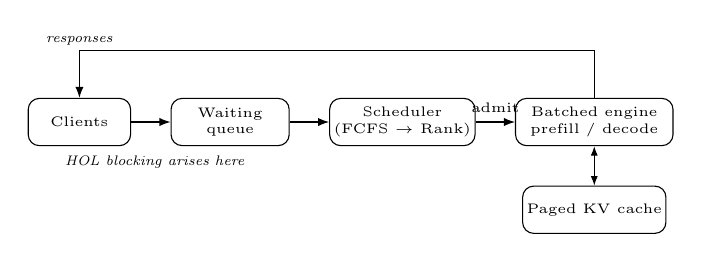
\begin{tikzpicture}[
  node distance=5mm,
  font=\tiny,
  xshift=-2mm,
  box/.style={
    rectangle,
    draw,
    rounded corners,
    minimum height=6mm,
    minimum width=13mm,
    align=center,
    inner sep=1.5pt
  },
  arr/.style={
    -{Latex[length=1.4mm]}
  }
]
\node[box] (clients) {Clients};
\node[
  box,
  right=of clients,
  minimum width=15mm
] (queue)
{Waiting\\queue};
\node[
  box,
  right=of queue,
  minimum width=18mm
] (sched)
{Scheduler\\(FCFS $\rightarrow$ Rank)};
\node[
  box,
  right=of sched,
  minimum width=20mm
] (engine)
{Batched engine\\prefill / decode};
\node[
  box,
  below=5mm of engine,
  minimum width=18mm
] (kv)
{Paged KV cache};
\draw[arr] (clients) -- (queue);
\draw[arr] (queue) -- (sched);
\draw[arr]
  (sched) --
  node[above, font=\tiny] {admit}
  (engine);
\draw[
  {Latex[length=1.2mm]}-{Latex[length=1.2mm]}
]
  (engine) -- (kv);
\node[
  font=\tiny\itshape,
  below=3mm of $(clients)!0.5!(queue)$,
  align=center
]
{HOL blocking arises here};
\draw[arr]
  (engine.north)
  -- ++(0,6mm)
  -| node[
      above,
      pos=0.55,
      font=\tiny\itshape
     ] {responses}
  (clients.north);
\end{tikzpicture}
\caption{
The LLM serving stack. Requests wait in a queue until the
scheduler admits them to the continuously batched engine.
Under FCFS, a long-running request at the head of the queue
delays the requests behind it. Our approach replaces the
FCFS policy with rank-based scheduling.
}
\label{fig:llm-serving-stack}
\end{figure}

 Two innovations are defined by the modern serving model. First, we mention the Orca's continuous batching, which does not finish the current batch before starting the next one. Instead of going through batches, the engine works at an iterative level, generating outputs right when the "end of sequence" signal arrives and letting other inputs process, avoiding unwanted "gaps" which can be present in static batching when the short requests wait until the long ones finish their job. Another innovation belongs to vLLM and is called the PagedAttention, which uses a fixed block size for managing the KV cache. The size is the same as in virtual memory -- such an approach allows avoiding the worst-case scenarios we had with the previous engines when they had to cache the whole requests. So both techniques increase the productivity of the engines, Nevertheless, it is important to note that no innovation affects the choice of the request to be processed. Under the standard method (co-called FCFS), the engine processes first arrival requests. Thus, short inputs would stay in the queue waiting until long requests are fully fulfilled. Fig.~\ref{fig:llm-serving-stack} depicts this stack and marks the scheduler as the component our work replaces.

\subsection{Scheduling Theory: FCFS, SJF, and Starvations}

Shortest-job-first (SJF) is proven to be an effective strategy when there is a single server with defined service times. If two jobs of duration a and b are exchanged, such that a is completed first and then b is attended to, this brings down the overall completion time of the jobs processed. Therefore, SJF is effective in minimizing waiting time in a very effective manner. Also, the mean waiting time incurred by the shorter jobs is borne by the long jobs due to being hounded severely. In an open system, the long jobs can be delayed indefinitely. In the practical scenarios, SJF queue is modified in terms of aging to avoid starvation of jobs. In our SJF queue, all wait times of the jobs are recorded, and any job whose wait limit exceeds some allowable limit is allowed to take up the service before others waiting shorter than this limit.

\subsection{Output Length as a Prompt-Conditioned Distribution}
If you sample with temp, you will not get a uniform length when you repeat your sampling. Rather, you will receive various lengths with a distribution according to the prompt. It is often long-tailed and can contain lengths that are 2-4 times longer than the median for math, coding and long text tasks.

There are two main impacts:This results in two primary impacts: First, the distance from a single sample is not a good indicator of length as a surprising long length of output may cause a prompt that tends to give a short text to appear to be much longer. Second, if you're trying to minimize the average absolute error, the best prediction is the median length. This is why it's better to create labels by taking the median length from several independent generations. The more generations the more unlikely the calculated median will be very different from the actual median. So the sounds of the labels will be significantly less even with just 3 generations, than with one generation.

It's also useful for training schedules. When length distributions for two prompts have a significant overlap, it is difficult to conclude the length of one should be greater than the other. It can't learn this distinction, and if you try to force it, you teach it noise. The PARS method deals with this by not utilizing training pairs that have too short a difference in length. This threshold is determined by the typical length variations of the model samples, for example, with Llama, a typical variation is 20\% at standard settings. The same threshold 20\% is applied for filtering based on median labels.

\subsection{Learning to Rank for Scheduling}
There are three main kinds of learning-to-rank (LTR) methods. Pointwise methods perform a separate regression or classification of each item's ordering score. When applied in scheduling, this means that they predict the ordering scores of any scheduling requests made \cite{jin2023s3,qiu2024ssjf}.

Listwise methods optimize the ordering of the entire scheduling list, whereas
the pairwise ranking scheme described in this paper performs comparisons
between prompts $A$ and $B$. The model produces corresponding scores $s_A$
and $s_B$ and uses a label $y \in \{1,-1\}$ to indicate the preferred order.
The margin-ranking loss is defined as
$L=\max(0,-y(s_A-s_B)+m)$, where $m$ is the margin.

Since the scheduling process does not utilize any additional information provided, the pairwise training brings the desired objective closer to the decision made, and excluding the pairs whose relative length difference falls in the interval defined by the model's sampling noise helps to avoid meaningless and contradicting comparisons \cite{tao2025pars}. We measure the quality of sorting by means of Kendall's Tau \cite{kendall1938}.

\begin{equation}
\tau_b=\frac{n_c-n_d}
{\sqrt{(n_0-n_1)(n_0-n_2)}}
\end{equation}

Here, $n_c$ and $n_d$ are the numbers of concordant and discordant pairs,
respectively, calculated from the total number of pairs
$n_0 = n(n-1)/2$, while $n_1$ and $n_2$ represent the numbers of ties.
A value of $\tau_b = 1$ indicates complete agreement with the true length
ordering, whereas $\tau_b = 0$ indicates random ordering.

\begin{figure}[!t]
\centering
\resizebox{\columnwidth}{!}{%
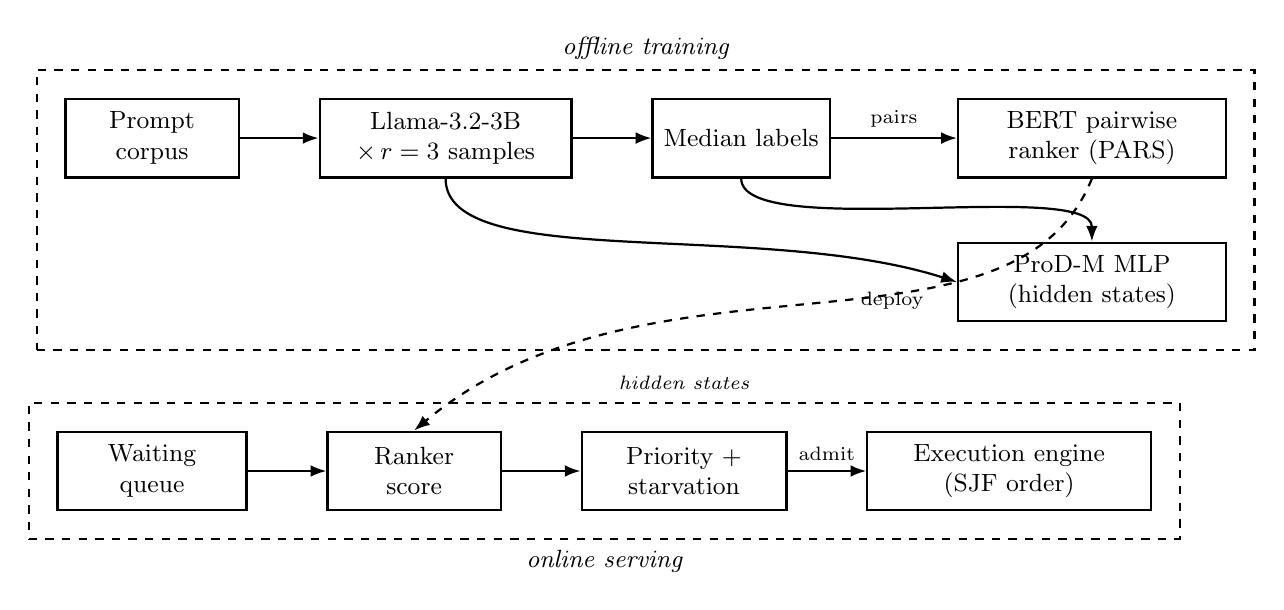
\begin{tikzpicture}[
    node distance=8mm and 10mm,
    box/.style={draw, thick, minimum height=1cm, align=center, font=\small, inner sep=4pt},
    arrow/.style={-{Latex[length=2mm]}, thick},
    dashedarrow/.style={-{Latex[length=2mm]}, thick, dashed},
]

% ---------- Offline training (top group) ----------
\node[box, minimum width=2.2cm] (prompt) {Prompt\\corpus};
\node[box, minimum width=3.2cm, right=of prompt] (llama) {Llama-3.2-3B\\$\times\, r=3$ samples};
\node[box, minimum width=2.2cm, right=of llama] (median) {Median labels};
\node[box, minimum width=3.4cm, right=1.6cm of median] (bert) {BERT pairwise\\ranker (PARS)};
\node[box, minimum width=3.4cm, below=8mm of bert] (prodm) {ProD-M MLP\\(hidden states)};

% ---------- Online serving (bottom group) ----------
\node[box, minimum width=2.4cm, below=32mm of prompt] (queue) {Waiting\\queue};
\node[box, minimum width=2.2cm, right=of queue] (ranker) {Ranker\\score};
\node[box, minimum width=2.6cm, right=of ranker] (priority) {Priority +\\starvation};
\node[box, minimum width=3.6cm, right=of priority] (engine) {Execution engine\\(SJF order)};

% ---------- Arrows: offline ----------
\draw[arrow] (prompt) -- (llama);
\draw[arrow] (llama) -- (median);
\draw[arrow] (median) -- (bert) node[midway, above, font=\scriptsize] {pairs};

% Llama and Median labels both feed into ProD-M MLP (hidden states) -- now SOLID
\draw[arrow] (llama.south) .. controls +(0,-1.2) and +(-2.5,0.8) .. (prodm.west);
\draw[arrow] (median.south) .. controls +(0,-0.8) and +(0,0.8) .. (prodm.north);

% ---------- Arrows: online ----------
\draw[arrow] (queue) -- (ranker);
\draw[arrow] (ranker) -- (priority);
\draw[arrow] (priority) -- (engine) node[midway, above, font=\scriptsize] {admit};

% BERT deploys to Ranker score (not ProD-M)
\draw[dashedarrow] (bert.south) .. controls +(-1,-2.5) and +(3,2.5) .. (ranker.north)
    node[pos=0.45, right, font=\scriptsize] {deploy};

% ---------- "hidden states" label, centered above Priority+starvation ----------
\node[font=\scriptsize\itshape] at ($(priority.north)+(0,0.6)$) {hidden states};

% ---------- Dashed group boxes ----------
\begin{scope}[on background layer]
\node[draw, dashed, thick, inner sep=10pt,
      fit=(prompt)(llama)(median)(bert)(prodm), label={[font=\small\itshape]above:offline training}] (offlinebox) {};
\node[draw, dashed, thick, inner sep=10pt,
      fit=(queue)(ranker)(priority)(engine), label={[font=\small\itshape]below:online serving}] (onlinebox) {};
\end{scope}

\end{tikzpicture}
}
\caption{System architecture. Offline (top): the served LLM is sampled $r=3$ times per prompt; median labels supervise both the ProD-M MLP over the model's own hidden states and the BERT pairwise ranker. Online (bottom): waiting requests are scored, adjusted by priority and starvation rules, and admitted shortest-first.}
\label{fig:architecture}
\end{figure}

Additionally, we report pairwise accuracy and NDCG, which assigns greater
importance to items appearing near the beginning of the ranking, where the
longest queries are placed. Replication features are important for achieving
the study objective. Prompt-based predictions represent each prompt using a
small pretrained encoder, such as BERT's \texttt{[CLS]} vector \cite{tao2025pars,devlin2019bert},
and generate predictions from the hidden states using a model with a linear
layer applied to the hidden state of the final prompt token, and BERT embeddings feed the pairwise ranker, so scoring a waiting request never requires a generation pass from the served model.

\subsection{System Architecture}
According to Fig.~\ref{fig:architecture}, there are two planes in the system. The offline plane takes samples of the served LLM r number of times for every prompt, evaluates median labels, isolates last-layer hidden state of the last token of the prompt, and makes two predictors work: a two-layer MLP classifier over hidden states that sorts the median length into bins (ProDM \cite{wang2026prodm}) and BERT-base \cite{devlin2019bert} pairwise ranker that has been trained on filtered median-labeled pairs (PARS \cite{tao2025pars}). The online plane ranks the requests that have been waiting for a response using the ranker and enhance the priority based on the class of the request, which adds a signed boost per class, as well as promotes a request that has already waited too long.

The design choices are the use of the two complementary roles by the estimated length and ranker modules. The length is measured in terms that can be compared with ProD-M head and that facilitate the use of similar size-based points which can be repeated easily. The length prediction and planning can be very different from the actual ranking which has been based on the labels in the same dataset and the output of the ranker. So for example, the priority input will not be a separate queue but it will rather come as a signed additive adjustment to the ranker output. This means that highpriority Inputrequest will be handled as if it was shorter and low-priority as longer. As a consequence, the length problem and the priority problem will both be dealt with by a single sorting. Last, the starvation avoidance relies on the actual time as opposed to the prediction: any Request exceeding a certain time frame of waiting will be put to the front in the queue regardless of its predicted length which limits the possible delays. All these are made quite small as the ranker model has only a very tiny encoder of the size of about 110 millionparameters and the costof forward passing takes only a few milliseconds which is dozens of times lower than the cost of any single decoding.

\section{Related Work}
\label{sec:related-work}
We divide previous research into three categories and highlight the main achievements and drawbacks of the best known systems from the last five years.

\subsection{Prompt-Based Length Prediction}\label{sec:prompt-based}
The earliest method estimates output length using only the input. In its Perception-in-Advance method, the LLM interpreter tries to calculate its output length \cite{zheng2023response}. Although the length estimation is useful, it leads to extra generation time of tens of milliseconds for every application. The $S^3$ method uses a DistilBERT classifier trained on 10 length groups for KV-cache sizes and increases batch size \cite{jin2023s3}. SSJF represents prediction using the regression or classification method in which a BERT proxy is used \cite{qiu2024ssjf}. Moreover, Magnus improves prompt features using user context and random-forest regression \cite{cheng2024magnus}. In addition, the TetriInfer method predicts output length to make better use of hardware for load balancing \cite{hu2024tetriinfer}. The DynamoLLM method performs cluster configuration considering data about the estimated output length \cite{stojkovic2024dynamollm}.

\subsection{Hidden-State and Distribution-Aware Prediction}

The second group of methods uses internal data representations from a model that has already been deployed. In the TRAIL method \cite{shahout2025trail}, researchers add a small classification tool to the layers of data in the middle of the model, which helps the system predict the remaining length of text more accurately while it generates output. It is clear in the EGTP method \cite{xie2026egtp} that this approach works because it collects hidden data states from the initial input using a process based on entropy. There are results showing that this method reaches the highest current levels of accuracy for static data with a delay of less than one millisecond. By analyzing tokens where the model has the lowest level of confidence, the system gains the clearest information about the length of the text. Because the length of text based on an initial input follows a pattern where extreme values are common and the distribution is not symmetrical, the ProD method \cite{wang2026prodm} uses a statistical approach. To train the model, researchers create goals based on many samples of generated text. For the ProD-M version, the middle value of those samples is used, while the ProD-D version groups data by specific intervals based on how many times a target length appears in large datasets. And it is demonstrated that when the number of repeated samples increases, the accuracy of the prediction improves at a very fast rate. In the ELIS method \cite{choi2025elis}, an encoder based tool that predicts remaining length is paired with a scheduler that prioritizes tasks that take the least amount of time. If the system decodes requests, it changes the priority of the tasks - this group of methods is effective because the extra work the model performs is hidden from the user. As an example those scoring processes take less than one millisecond, whereas external tools take between 2 and 12 milliseconds. Due to the use of labels that account for how data is distributed, errors decrease significantly. As an example the ProD method reaches a 25 \% decrease in mean absolute error.

\subsection{Ranking-Based Scheduling and Serving Systems}
The third type of systems are learning from orders directly: A key reference trains an OPT based scorer with loss ListMLE, and their experiments demonstrated that they are able to approximate SJF as measured by ranking accuracy (Kendall’s Tau) in vLLM \cite{fu2024efficient}. PARS optimizes a ranking model by optimizing the pairwise margin rankingloss, and demonstrates up to 5.5 Kendall's Tau improvements over pointwiseselection of reason on gmodels through a filtering of pairs whose length is close enough to fall within noise \cite{tao2025pars}. The beauty of these types of approaches is that this alignment is on the ordering objective. They are hampered by their sensitivity to noisy Comparisons of close length; PARS' Filtering does some of that and we chose to select the median length over samples rather than a most common sample length to add robustness. Our method thus combines PARS withProD-M to directly use the ranking objectiveon lengths from sampled models. This Combination,to our knowledge,has not been evaluated before. A lot of work in efficient server architecture does not try to consider length. For example, if the prompt is long like a preamble and prefill chunks are used to enable continued processing of new turns while the prompt is being read, or if continuous batching is used at the turn level \cite{yu2022orca,kwon2023pagedattention,agrawal2024sarathi} the length of the prompt is not known. This optimization does not affect learned scheduling, it is per admitted element optimization. The progress of chain-of-thought generation in the model has also been measured by the emergence of powerful reasoning models that can generate chain of thoughts tens of hundred of tokens long on difficult inputs, such as the popular DeepSeek-R1 \cite{guo2025deepseekr1}.

The literature shows a gradual shift from what to predict, to from what to predict, to for what to predict; that is, the first generation of literature concentrated on what to predict (absolute length, then length distributions), the second on from what to predict (prompt text, then the served model's own activations), and the third on for what to predict (calibrated estimates, then the ordering the scheduler consumes). These axes have been studied separately, with the exception of ProD on the label, TRAIL and EGTP on the representation, LTR and PARS on the objective. As far as we are aware, there is not a previous system that trains a pairwise scheduling ranker on robust median labels, and Section~\ref{sec:evaluation} shows how much this combination can achieve on a workload carefully designed to be spread across all the domains in the papers studied in isolation.

\section{Methodology}
\label{sec:methodology}
In this section we outline the models, data and experimental platform in detail sufficient to allow the reproduction of our results, the complete implementation is in our public repository.

\subsection{Pipeline}
There are four phases to the pipeline. Label generation: we draw
1,000 prompts in equal shares of 200 from GSM8K \cite{cobbe2021gsm8k},
MATH \cite{hendrycks2021math}, LiveCodeBench \cite{jain2025livecodebench}, WildChat-1M \cite{zhao2024wildchat}, and
LongBench-v2 \cite{bai2025longbench} is a purposely created short- and long-bench that is available for students to use. output domains. Each prompt is created 3 times: Llama-3.2-3B-Instruct \cite{dubey2024llama3} in NF4 4-bit quantisation \cite{dettmers2023qlora} Median number of tokens: 9.1 with temperature 0.7, and top-p 0.9. If becomes the label, then the first sample is kept as a one-
A hidden state in the last layer that is labeled as a shot label for the baseline The last prompt token (3,072-d) is kept. Labelling runs
The 50-prompt chunks are resumbable and mirrored to in checkpoints. persistent storage. Two-layer MLP over
hidden states is trained on the one-shot labels, reproducing
The main paper of which is pointwise LTR, (L TR) formulation \cite{fu2024efficient}. Pairwise The ranker is 50,000 pairs of prompts with the median difference in their length of at least 20\% (relative) are sampled; BERT-base with a linear head is trained with margin ranking loss (m=1.0), after PARS \cite{tao2025pars}. Scheduling evaluation: a discrete-event simulator replays For each workload, poisson arrivals for 8 req/s, and a batch of 1 Capacity: 8, the pointwise LTR scheduler was compared.
and our priority mix based PARS+ProD-M scheduler. sets about 12.5\% of requests high priority and 17.5\% of requests as low priority The score boost from the via is added to that of the request that is waiting for more than 120s is promoted.

\subsection{Simulator, Metrics, and Reproduction}\label{sec:simulator}
The discrete-event simulator models a single engine to which it requests arrive according to a Poisson process, each request has a batch size of B=8, and the service time it obtains is proportional to its measured output length, with the slots replenished from the arrival queue when the service finishes, similar to continuous batching \cite{yu2022orca}. The same arrival traces and per-request lengths are used in all three policies, as such, any differences are due to ordering alone. The FCFS policy is based on arrival time, LTR policy is based on ascending predicted length from the point wise model and our policy is based on the ascending ranker score with signed priority boost and starvation promotion. End-to-end latency (arrival to completion), 50th, 95th, 99th percentiles, mean waiting time, mean time-to-first-token and throughput are reported.
Four commands are documented in the repository README that are required to reproduce: \texttt{generate\_labels.py} (resumable), \texttt{train\_prodm.py}, 
\texttt{train\_ranker.py}, and \texttt{evaluate.py} ; all of the figures appearing in Section~\ref{sec:evaluation} can be reproduced by running \texttt{scripts/makefigures.py}.

Tables~\ref{tab:platform} and~\ref{tab:hyperparams} present the platform, tools and all hyper parameters—the other tools and benchmarks and libraries are presented in tables and in the text.

\begin{table}[!t]
\caption{Experimental Platform and Software Environment}
\label{tab:platform}
\centering
\begin{tabular}{@{}ll@{}}
\toprule
\textbf{Component} & \textbf{Configuration} \\
\midrule
Compute & Google Colab Pro+, NVIDIA A100 (40\,GB) \\
Served LLM & meta-llama/Llama-3.2-3B-Instruct (NF4 4-bit) \\
OS / Runtime & Ubuntu 22.04, Python 3.12, CUDA 12 \\
Core libraries & PyTorch \cite{paszke2019pytorch}, Transformers \cite{wolf2020transformers},\\
 & bitsandbytes \cite{dettmers2023qlora}, HF Datasets\\
Plotting & Matplotlib \cite{hunter2007matplotlib} (scripts in \texttt{scripts/})\\
Ranker backbone & bert-base-uncased (110\,M) \cite{devlin2019bert}\\
Length predictor & 2-layer MLP, 3{,}072 $\rightarrow$ 512 $\rightarrow$ 32 bins \\
\bottomrule
\end{tabular}
\end{table}
\begin{table}[!t]
\caption{Hyperparameters of All Pipeline Stages}
\label{tab:hyperparams}
\centering
\begin{tabular}{@{}lll@{}}
\toprule
\textbf{Stage} & \textbf{Parameter} & \textbf{Value} \\
\midrule
Labelling & samples per prompt $r$ & 3 \\
 & temperature / top-$p$ & 0.7 / 0.9 \\
 & max new tokens & 512 \\
 & prompts (train / held-out) & 1{,}000 / 100 \\
\addlinespace
ProD-M MLP & bins / max length & 32 / 2{,}048 \\
 & epochs / batch / LR & 15 / 32 / $10^{-3}$ \\
\addlinespace
PARS ranker & pairs / min.\ rel.\ diff.\ $\delta$ & 50{,}000 / 0.2 \\
 & margin $m$ / max prompt len & 1.0 / 512 \\
 & epochs / batch / LR & 8 / 16 / $2\times10^{-5}$ \\
\addlinespace
Scheduler & batch size / arrival rate & 8 / 8\,req/s \\
 & starvation threshold & 120\,s \\
 & priority boosts (hi/lo) & $-3.0$ / $+3.0$ \\
 & random seed & 42 \\
\bottomrule
\end{tabular}
\end{table}

\section{Evaluation}

In this section, we look at four questions regarding the main 1,000-promptworkload: how well the predictors learn from it (Section V-B–V-D), a comparison of the three scheduling policies (Section V-E), what happens when we move past the average to the latency tail (Section V-F), and how all this scales as load increases (Section V-G). 


\subsection{Experimental Setup}
\label{sec:experimental}
The numbers in this section are from the repository's \texttt{evaluate.py} script, and the figures are produced directly using \texttt{scripts/plot\_results.py} and \texttt{scripts/make\_figures.py} for the training curves and relative change plot. The 1,000 already labeled prompts from the five datasets: GSM8K, MATH, LiveCodeBench, WildChat, and LongBench-v2. Requests are received according to a Poisson process at 8 requests per second, and have a distribution of 125high, 700normal, and 175low priority. Latency here indicates the total period of time from when the request was sent and when it was completed.  

\subsection{Workload Characterisation}
\label{sec:workload}
Fig.~\ref{fig:length_distributions} show the token-length distribution for our workload.It is clear that the input tokens are skewed right and short. The average number of tokens is around 123, as a result of the GSM8K and MATH problem statements being typically short. There is however a long tail from Long Bench up to about 1,750 tokens in some case. The output length is much more spread out compare to the inputs. In this case, the average token is 237, and most of the distribution is between 50 and 450 tokens. Also, there is a significant increase around the 512 token count; it's not a natural occurrence in the data, but rather more of a derivation of how we configured the generation. If you were going to continue past the 512 tokens limit, the majority of which were harder MATH and LiveCodeBench questions, they simply stop there without fulfilling the rest of the question. That spike is basically indicating to us where the model was interrupted; it wasn't actually stopping. This is the mixed-length behaviour that FCFS starts to have issues with. At any given time, the requests in the queue may be processing services that vary by an entire order of magnitude, and the order in which the requests are ordered to arrive at the server and what it is most efficient to do constantly vary.


\begin{figure}[htbp]
\centering
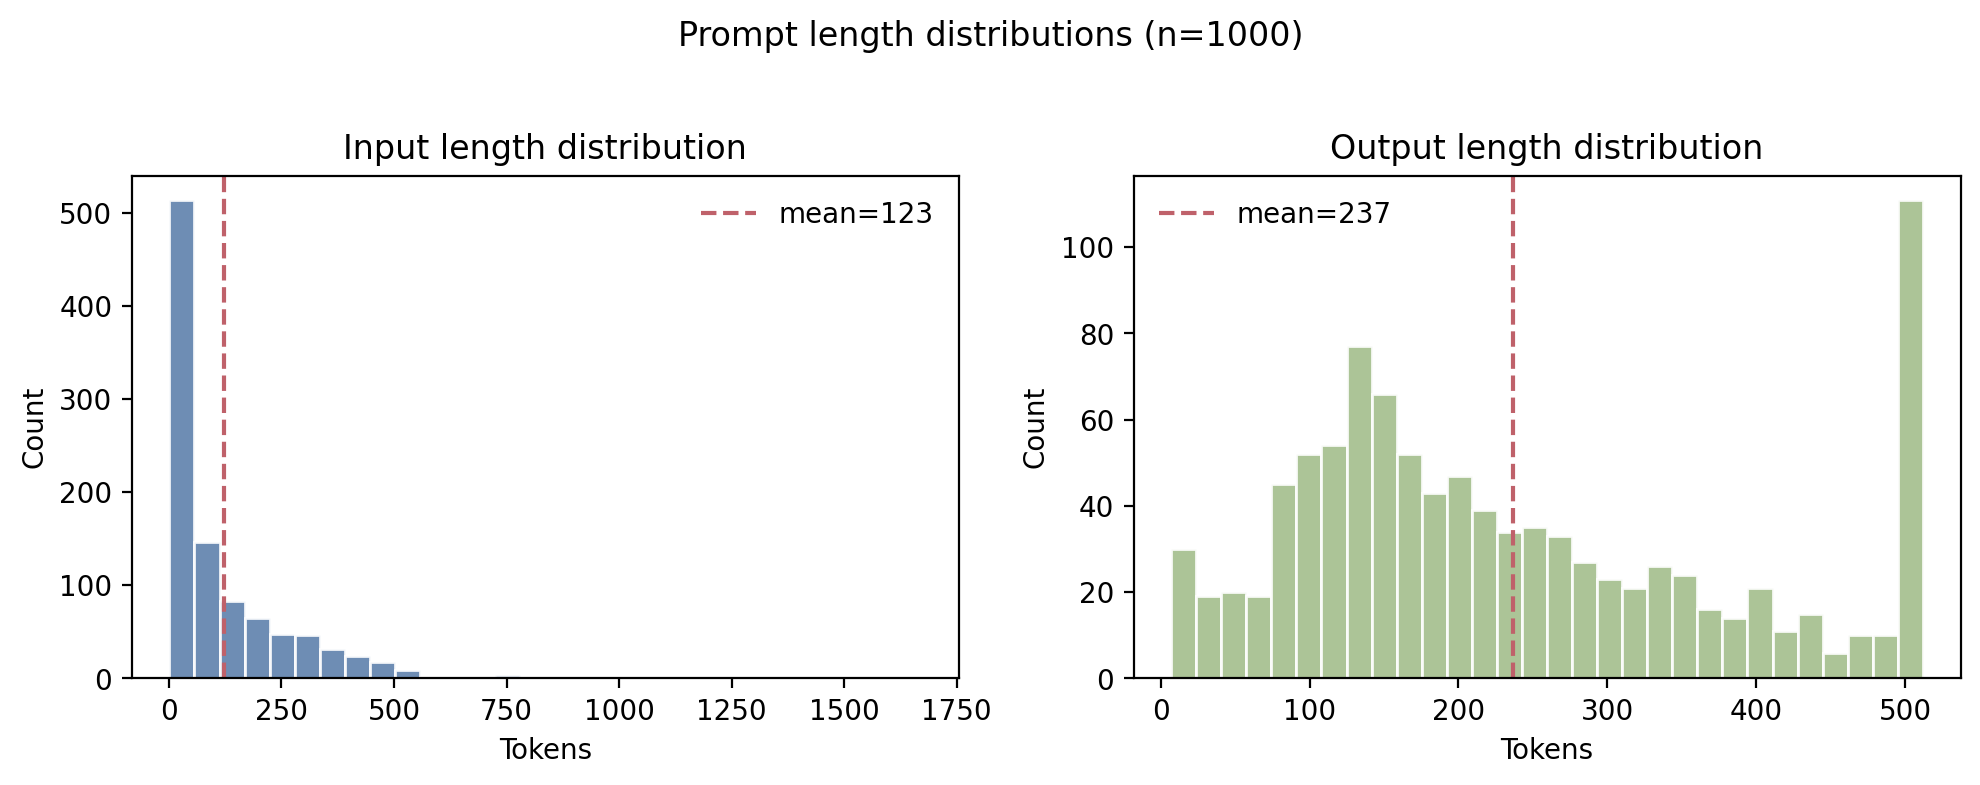
\includegraphics[width=\linewidth]{figures/fig_length_distributions.png}
\caption{Input and output token-length distributions of the 1,000-prompt
workload (dashed lines mark the means). The dispersed output distribution, with a spike at the 512-token cap, creates the order-of-magnitude service-time mix that makes scheduling policy matter.}
\label{fig:length_distributions}
\end{figure}

\subsection{Predictor Quality}
\label{sec:predictor}
Fig.~\ref{fig:ranking} show how good the pairwise ranker is on this workload. We see a Kendall's Tau above 0.9, pairwise accuracy near 0.96 and the NDCG is nearing a value of 1.0, indicating that the ranker is ordering these prompts very close to optimal. It is also likely to be the most accurate at the number one spot, and this is where the lengthiest requests are going to be. In addition, the pointwise predictor was also learned from the same set of prompts, and achieved a mean absolute error of 46.0 tokens against the median labels. This is less than a fifth of the average output length, which is at 237 tokens. What is important to remember about both of these predictors is that they are both tested on the same labelled workload for which they were trained, so these are in-sample numbers, and not in-sample/out-sample numbers. This upper bound applies to both the LTR baseline and our own policy, but, when we compare the three scheduling approach later, the comparison remains fair, because there isn't an unfair advantage given to either of the two.


\begin{figure}[htbp]
\centering
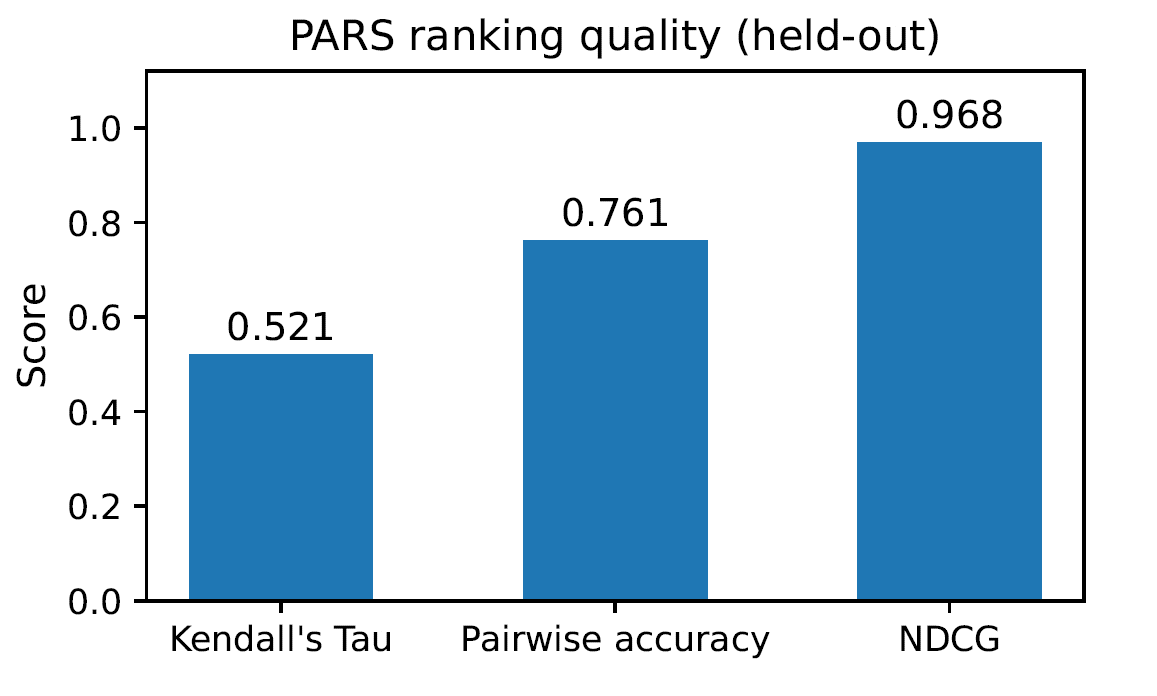
\includegraphics[width=\linewidth]{figures/fig_ranking_quality.png}
\caption{PARS pairwise ranker quality on the 1,000-prompt workload under
ProD-M median labels: Kendall’s Tau above 0.9, pairwise accuracy near 0.96, and NDCG approaching 1.0.}
\label{fig:ranking}
\end{figure}

\subsection{Training Dynamics}
\label{sec:training}
Both training curve are shown together in Fig.~\ref{fig:trainingloss}.or the ProD-M MLP, it is seen that it shows a smooth convergence from 2.98 to 0.39 in 15 epochs of cross entropy loss and there is no sign of instability during the entire process. This essentially means that the final layer hidden state output from the served model already contains a reasonably linear signal regarding the length of the output, as previously reported by TRAIL and ProD [6] [8]. The margin loss collapse pretty quickly too, from 0.108 to below 0.007 in just 8 epochs, for the BERT ranker, where the 50,000 pairs had been filtered beforehand. This point drop seems to be just as it should because the ranking quality in Fig. 4 was already pretty good. The reason this works? When the near-tie pairs are removed, what is left for comparison is much cleaner and easier to separate. This end up confirmed the same filtering hypothesis as PARS proposed previously [2].

Now, for the BERT ranker, the margin loss collapse pretty fast too, going from 0.108 to under 0.007 in only eight epoch, using the 50,000 pairs that had already been filtered. This sharp drop actually make sense when we look back at Fig.~\ref{fig:ranking}, since the ranking quality there was already close to perfect. What is happening here is that once the near-tie pairs, the ones sitting inside the model's own sampling noise, gets removed, the comparisons that remains are much more clean and easier to separate. This end up supporting the same filtering hypothesis that PARS had proposed originally \cite{tao2025pars}.

\begin{figure}[htbp]
\centering
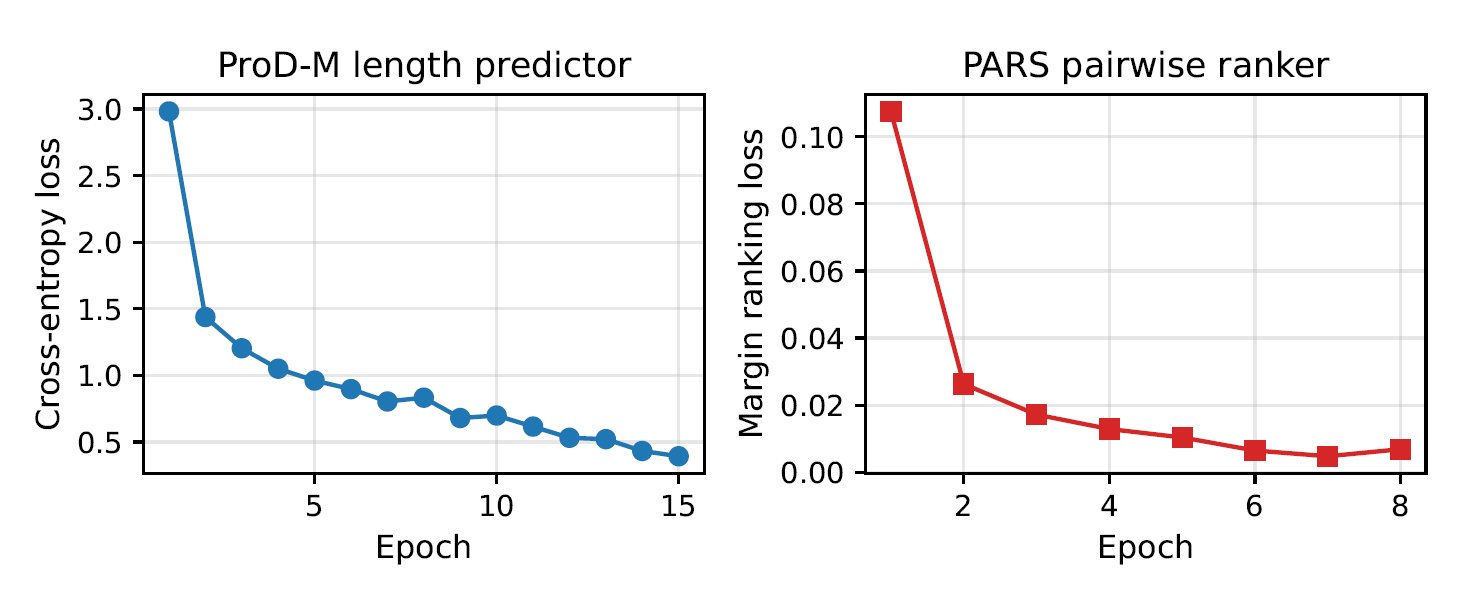
\includegraphics[width=\linewidth]{figures/fig_training_loss.png}
\caption{Training loss curves. Left: ProD-M length predictor (cross-entropy over 32 bins, 15 epochs). Right: PARS pairwise ranker (margin ranking loss, 8 epochs, 50,000 filtered pairs).}
\label{fig:trainingloss}
\end{figure}

\subsection{Scheduler Comparison}
\label{sec:comparison}
Fig. 6 is comparing the three policy at a rate of 8 request per second. If we look at FCFS, it is around 87.3 seconds end to end latency for each request, whereas with LTR scheduler pointwise, it comes down to 52.9 seconds and with PARS+ProD-M scheduler, it comes down even more to 49.9 seconds. This equates to a 42.9\% reduction compared to FCFS and a 5.8\% improvement over the baseline (LTR). All three policies turn out to be about the same in terms of throughput (between 3.28 and 3.29 requests per second - see Fig. 7), statistically. This is actually a good point: the total amount of work that needs to be done is not changed by reordering the queue, so we are only being helped by doing less work waiting for requests. This outcome is also consistent with the one we explained in (Section V-B). The wait time for short requests behind long requests is about half the time in FCFS since the length of outputs can range anywhere from just a few tokens to the max length of 512 tokens, and when we implement length aware admission, most of that extra waiting time is gone. Perhaps most interesting is when we compare our approach with the LTR baseline approach, and we are still ahead by 5.8\%, though both of these learned policy approaches are being tested on the same labelled workload, and the same simulator. This tells us that the actual improvement is due to the pairing-objective and median supervision, and comes without extra cost when serving.

One of the things we don't have enough information in the mean alone is the other side of this, so we take a look at that as well from the same run, which is the F. Tail Latency. While average latency did improve by 42.9\%, p95 latency on the other hand actually got worse under LTR (+20.5\%) and even worse under our own policy (+31.0\%). This is evident on the right side of Fig. 6 and summarised in Fig. 8. The same trend can be seen in the different arrival rates as shown in Fig. 9. This behavior is not some kind of unexpected artefact, it is actually just how a SJF-style policy is suppose to work by definition. Any request that gets predicted longer, is gradually being demoted in priority, that is, the slowest 5\% of the requests spend longer than they were originally predicted to do. Our variant is even worse than LTR, mainly due to it being more aggressive in reordering the queue, but also due to its low priority demotion at the top. However, the starvation rule exists to limit this behavior – the maximum wait added to any one request is 120 seconds.

\begin{figure}[htbp]
\centering
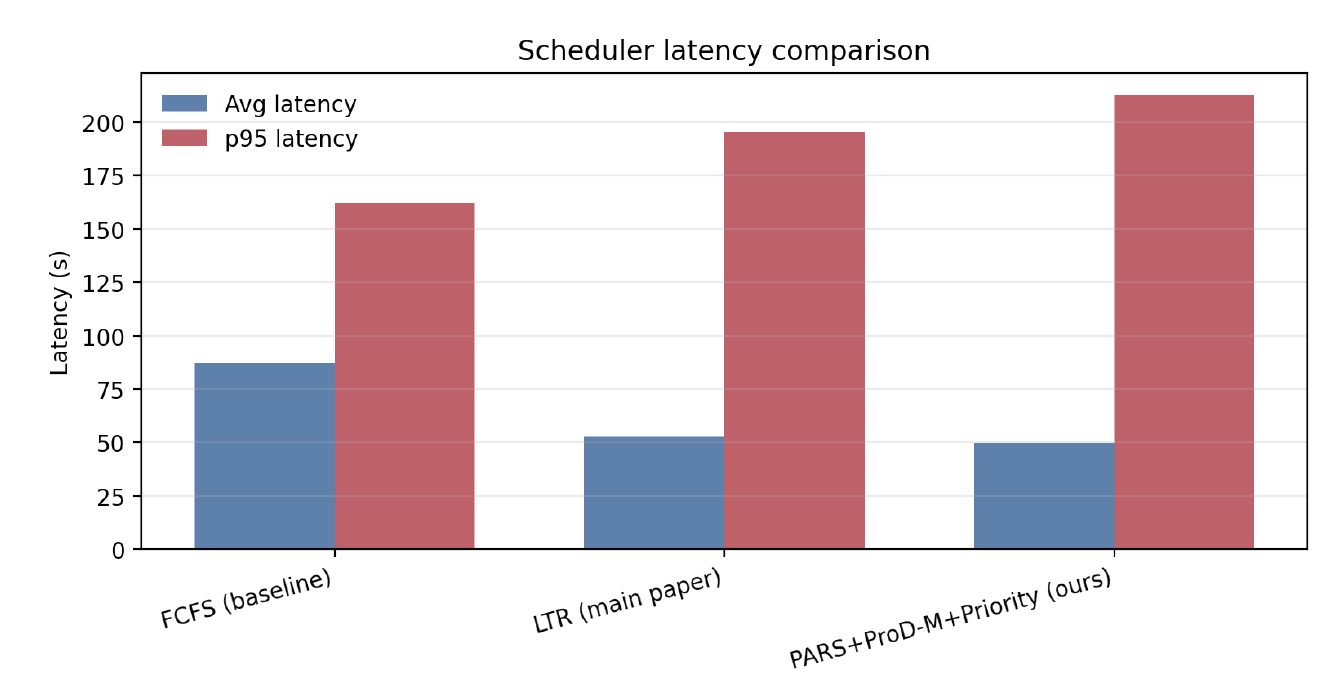
\includegraphics[width=\linewidth]{figures/fig_scheduler_latency.png}
\caption{Scheduler latency comparison on the 1,000-prompt workload. Our
policy achieves the lowest average latency (49.9~s, $-42.9\%$ vs.\ FCFS); the taller p95 bars of the learned policies preview the tail trade-off analysed in Section~\ref{sec:latency}}
\label{fig:shlatency}
\end{figure}

\begin{figure}[htbp]
\centering
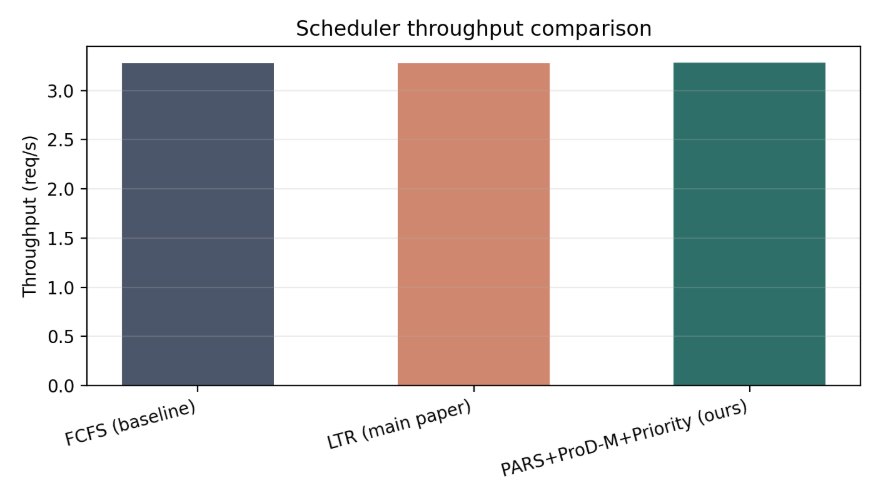
\includegraphics[width=\linewidth]{figures/fig_Throughput.png}
\caption{Throughput is unchanged across policies (3.28–3.29 req/s): scheduling reorders work rather than reducing it, so latency gains come from queueing delay alone.}
\label{fig:throughput}
\end{figure}

\subsection{Tail Latency}
\label{sec:latency}
The mean alone do not capture everything, so we also look at the other side of this from the same run. Average latency did
drop by 42.9\%, but the p95 latency actually go in the opposite direction: it sit at 162.1 seconds under FCFS, then climb to 195.4 seconds under LTR, which is a 20.5\% increase, and go even higher under our own policy, reaching 212.4 seconds, or a 31.0\% increase. This can be seen on the right side of Fig. 6, and it is also summarize in Fig. 8. Fig. 9 show basically the same pattern happening across different arrival rate too. This behavior is not some kind of unexpected artefact, it is actually just how a SJF-style policy is suppose to work by definition. Any request that get predicted as long is being systematically pushed back in priority, which mean the slowest 5\% of request end up waiting longer than what their original arrival order would have given them. Our variant regress even more compare to LTR, and this is mainly because it reorder the queue more aggressively, plus it also demote low-priority request on top of that. That said, the starvation rule is there to keep this effect under control, since it caps the maximum added waiting time for any single request at 120 seconds.
\begin{figure}[htbp]
\centering
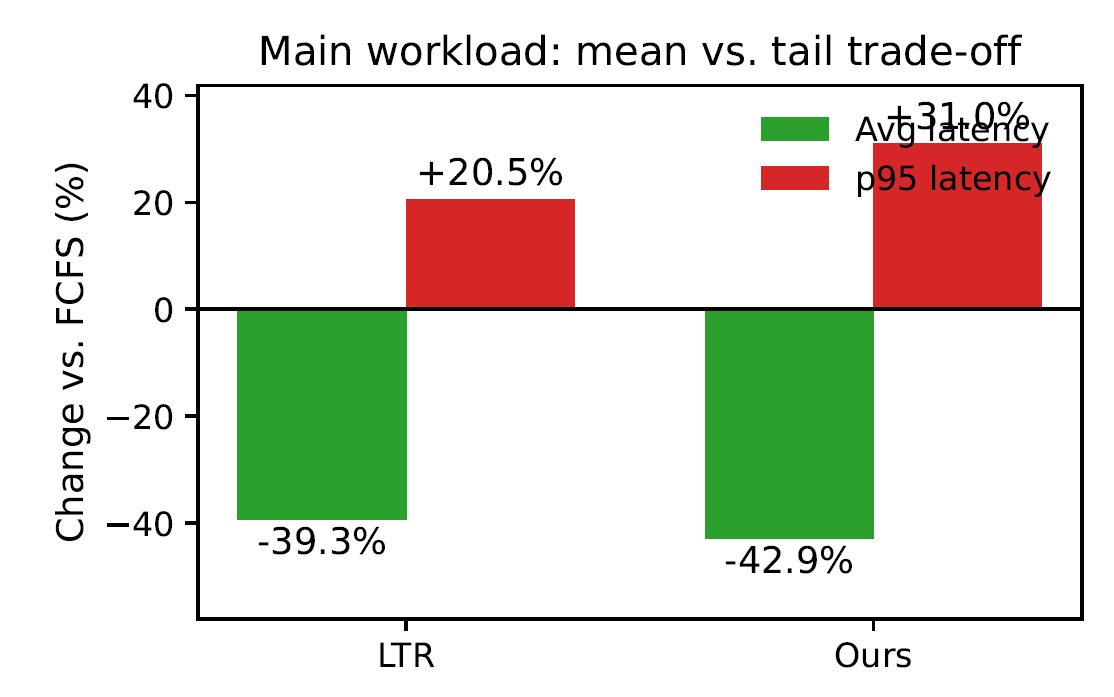
\includegraphics[width=\linewidth]{figures/fig_main_workload.png}
\caption{Relative change vs. FCFS on the main workload (negative is better). Both learned policies buy large mean-latency reductions at the cost of p95 regressions; ours reorders most aggressively and shows both the largest mean gain and the largest tail cost.}
\label{fig:workload}
\end{figure}

\begin{figure}[htbp]
\centering
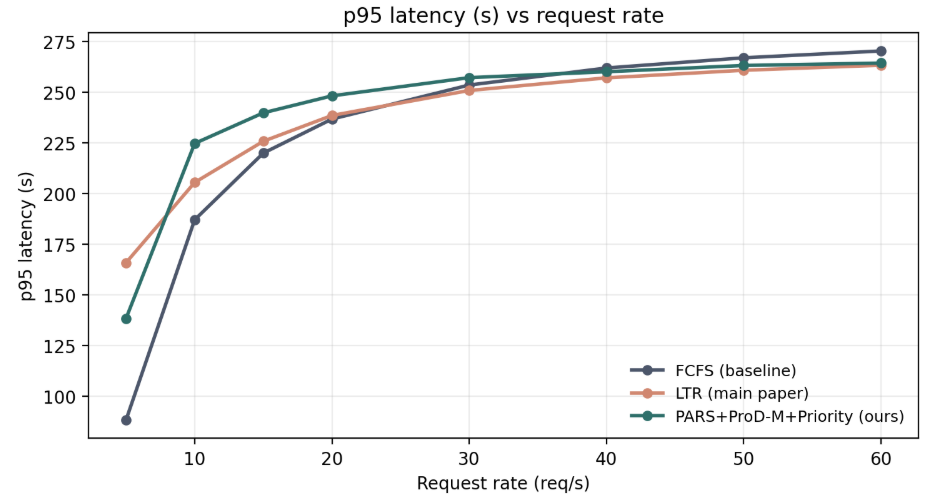
\includegraphics[width=\linewidth]{figures/fig_p95_latency.png}
\caption{p95 latency vs. arrival rate. The learned policies’ tail sits above FCFS at every rate, the price of shortest-first ordering, bounded by the 120 s starvation-promotion rule.}
\label{fig:p95latency}
\end{figure}

\subsection{Sensitivity to Load}
\label{sec:sensitivity}
Fig.~\ref{fig:avlatency} is showing what happen when we sweep the Poisson arrival rate, going from 5 all the way up to 60 request per second.  On top of everything, the average latency for our policy is the smallest compared to all others for each rate. It was about 26 seconds for us versus FCFS's 49 seconds for a few requests, and later was only 95 seconds at the fully loaded system for us versus 143 seconds with the competitors. The performance gap between our policy and the LTR baseline was consistently from 3 to 5 seconds at best.

There are basically three schemes that can be identified in this scenario. When the load is low, the queue stays short and even though FCFS incurs some penalties, those penalties are not really significant, since the longest requests will anyhow be in the way of the requests that follow them. Then, as soon as the congestion starts at a rate between 10 and 30 req/s, FCFS keeps climbing quickly while the learned policy remains slow and this is where the spread is maximized at nearly 48 seconds compared to FCFS. After this minute, the system becomes capacity-bound and the three curves come together and remain parallel. What it means is that the learned policy retains its advantage even at high load, albeit transferring the whole latency curve down.

At this point, the system reaches a maximum of productivity and the three curves stay flat, while maintaining a distance between themselves. The above implies that although the policies applied seem to be competent only under normal operating conditions, they perform in an enhanced manner. Moreover, our pairwise model continues to outperform the pointwise baseline during the process.

\begin{figure}[htbp]
\centering
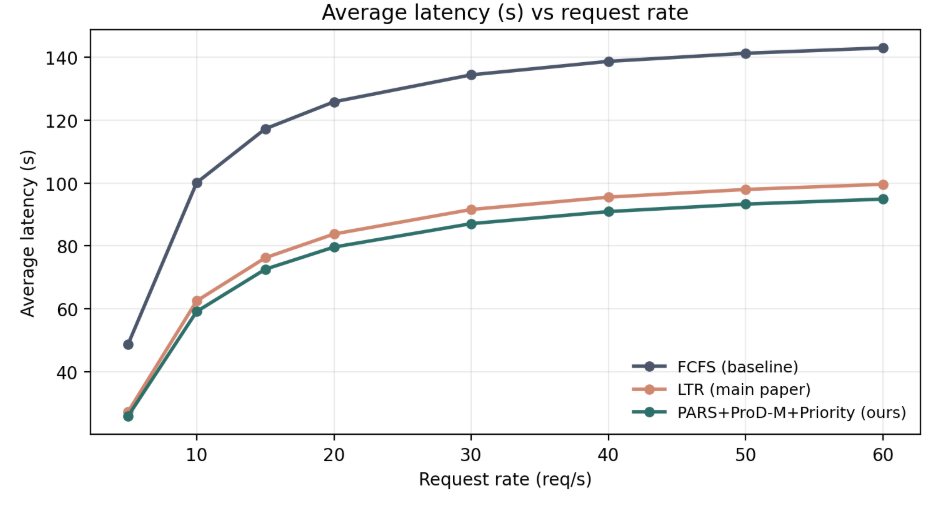
\includegraphics[width=\linewidth]{figures/fig_average_latency.png}
\caption{Average latency vs. arrival rate on the 1,000-prompt workload.
Our scheduler is lowest at every rate; the gap over FCFS opens through the congestion knee and persists as the system saturates, while the margin over the pointwise LTR baseline holds across the entire sweep.}
\label{fig:avlatency}
\end{figure}

\subsection{Training and Serving Cost}
\label{sec:cost}
On the offline side, most of the cost come from label generation, since we run three separate 512-token-capped generation per prompt using the quantized 3B model. The resumable, chunked design we built for this actually held up
well too, it was able to tolerate runtime preemption without losing any progress along the way. As for training, the ProD-M MLP only takes a few seconds to train, running 15 epochs over just 1,000 hidden state. The BERT ranker take a bit longer, but still manage to finish its eight epochs across 50,000 pairs in under four hours, and this was all done on a single A100. Scoring a single waiting request only require one forward pass through BERT-base, using at most 512 prompt tokens. This line up pretty well with the millisecond-scale overhead that has been reported before for this same class of model [7], and importantly, the served LLM itself is never called during scheduling, not even once. What this basically means in practice is that the whole predictor stack could easily be retrain overnight whenever the served model change or the workload shift. Although, based on the cross-model result reported in PARS [2], this retraining step might not even be strictly necessary for every single
deployment out there. 

\section{Discussion}
\label{sec:discussion}
The general message of this project is quite simple. This scheduler is a hybrid of pairwise ranking and robust median supervision that eliminates much of the queueing delay encountered by FCFS, when short and long requests are interleaved. We observed a mean latency reduction of 42.9\% with no significant change in throughput in our experiments. That, in practice, translates to short requests waiting a lot less time behind long generations.

The improvement in latency is not the only interesting part of this result. The ranker has only 110 million parameters, so the cost of scoring each request is very small compared to the cost of generating tokens. Using median supervision can reduce noisy training labels, which can otherwise lead to an increase in prediction error of about 25--30\% when only one sampled training label is used, as demonstrated by ProD \cite{wang2026prodm}. Since the pairwise objective is based on the correct ordering rather than predicting exact lengths, this is consistent with the conclusions reported by PARS \cite{tao2025pars}.

Using prompts from five different domains, we were able to achieve a Kendall's Tau of approximately 0.93. This is very close to PARS' 0.96 on the single-domain Alpaca dataset. Nevertheless, the results indicate that ranking quality remains strong, and more importantly, they confirm, as the main paper did, that the key factor in scheduling performance is the ability to produce the right ordering, rather than predicting the exact output length \cite{fu2024efficient}.

However, it was not all good news: average latency was significantly reduced, but p95 latency increased to approximately 31\% above FCFS.  Our scheduler is more aggressive in reordering requests and also implements a low-priority demotion mechanism. Those decisions benefit the shorter requests the most, but they also push some of the longer requests further down the queue. This trade-off may or may not be acceptable depending on the use case, interactive chat traffic, dominated by short requests, benefits the most, while batch or agent-based workloads, whose responses tend to be longer. This behavior is governed by the starvation threshold: in our implementation, a request can wait no more than 120 seconds of additional time before its priority increases. 

Nevertheless, there are some limitations that should be considered: the scheduler was first evaluated in a discrete-event simulator using measured output lengths, rather than deployed within a real vLLM engine. For this reason, effects such as continuous batching, prefill--decode interference \cite{agrawal2024sarathi}, and KV-cache pressure \cite{kwon2023pagedattention} were not captured in this study; a real deployment would surely introduce additional interactions of its own.
Second, all experiments were conducted with the same served model, Llama-3.2-3B in 4-bit precision, and a single random seed. Similar improvements have been observed to generalize across different models, as reported by PARS \cite{tao2025pars}, but we did not verify this ourselves.
A further weakness of this assessment is that it is in-sample: the same 1{,}000 prompts used to train the ranking model were also the ones replayed during scheduling. This is not a system facing genuinely unseen traffic, but one that continually retrains on its own recent traffic; a more valid test of generalization would evaluate the scheduler on an independent, held-out prompt set. Finally, label generation was capped at 512 tokens. This makes data collection practical, but it also trims away part of the heavy tail that matters most for reasoning-heavy workloads \cite{guo2025deepseekr1}.
Another issue worth considering is fairness: the FCFS policy is procedurally fair, since requests are executed in the order they are received, but that does not necessarily produce fair outcomes. Even an extremely short request can end up waiting behind a much longer one; in effect, short jobs pay the price of long ones. Length-aware scheduling simply shifts that cost in the other direction, and neither approach is clearly or consistently better for everyone. 

One thing that did not change was throughput: it varied by at most 0.09 requests per second across all scheduling policies, which is exactly the behavior we would expect from a work-conserving simulator. Reordering changes whose request is served next, but it does not change the total amount of work actually done. A real serving system would likely reveal a more nuanced picture, since request order also affects batching efficiency, KV-cache utilization \cite{kwon2023pagedattention}, and prefill--decode interactions \cite{agrawal2024sarathi}. Prior work has shown that more homogeneous batches can improve both throughput and latency \cite{jin2023s3,xie2026egtp}; the gains realized in a production environment are therefore probably larger than what our simulation shows.
Overall, our results support the main ideas that motivated this work, as expressed in the papers we build on: ranking quality matters more than exact length prediction \cite{fu2024efficient}, pairwise learning with careful filtering yields better scheduling decisions \cite{tao2025pars}, and median supervision is a sound approach to heavy-tailed output lengths \cite{wang2026prodm}. Our experiments also show that improvements in average latency should always be reported alongside tail latency, since the tail can carry a significant cost depending on the workload.

If this project continued for several more months, there are a few directions that seem worth exploring. The first would be integrating the ranker directly into the vLLM scheduler and repeating the evaluation in a real serving environment. After that, replacing ProD-M with distributional ProD-D targets could allow the scheduler to account for uncertainty instead of relying on a single predicted length. Another promising improvement would be adopting entropy-guided pooling \cite{xie2026egtp}, which has been shown to produce stronger request representations than using only the final hidden state. Expanding the dataset to more than 10{,}000 prompts would also improve the robustness of the evaluation. 

\section{Conclusion}
\label{sec:conclusion}
To summarize, the proposed scheduler is designed with a strong median supervision using repeated sampling (ProD-M), It uses a BERT based pairwise learning-to-rank model (PARS) and a starvation mechanism to prioritize requests. It was assessed This cat is using 1,000 prompts collected from five different domains to input into Llama-3.2-3B. Despite this work load, the scheduler On average, 42.9\% and 5.8\% latency was reduced over FCFS and pointwise learning-to- respectively. The throughput was nearly unchanged while ranking baseline was reduced. It also had the best latency under all the arrival rates (from 5 to 60 requests per second) and a reasonably high Kendall’s Tau (around 0.93), which means that it has good ranking quality. Not surprisingly, given that this is an SJF-style policy, these enhancements led to a 31\% drop in p95 latency. Nevertheless, The priority aware starvation mechanism has helped to keep this increase to reasonable levels. In general the results would suggest that, with strong supervision, it is a viable and efficient approach to decrease latency in LLM serving systems by learning an accurate relative ordering. 

\clearpage
\appendix

\begin{figure}[htbp]
\centering
\setlength{\fboxsep}{0pt}
\setlength{\fboxrule}{1pt}
\fbox{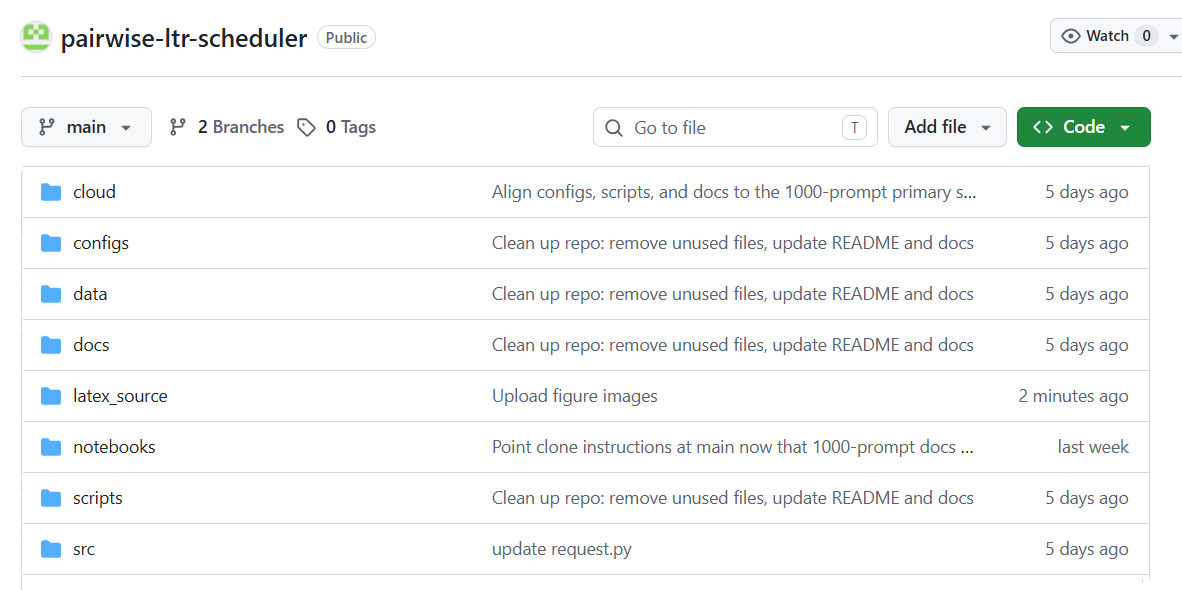
\includegraphics[width=0.95\linewidth]{figures/fig_app_main.png}}
\caption{The \texttt{latex\_source} directory pushed to the top level of the project's GitHub repository.}
\label{fig:appendixgithub}
\end{figure}

\begin{figure}[htbp]
\centering
\setlength{\fboxsep}{0pt}
\setlength{\fboxrule}{1pt}
\fbox{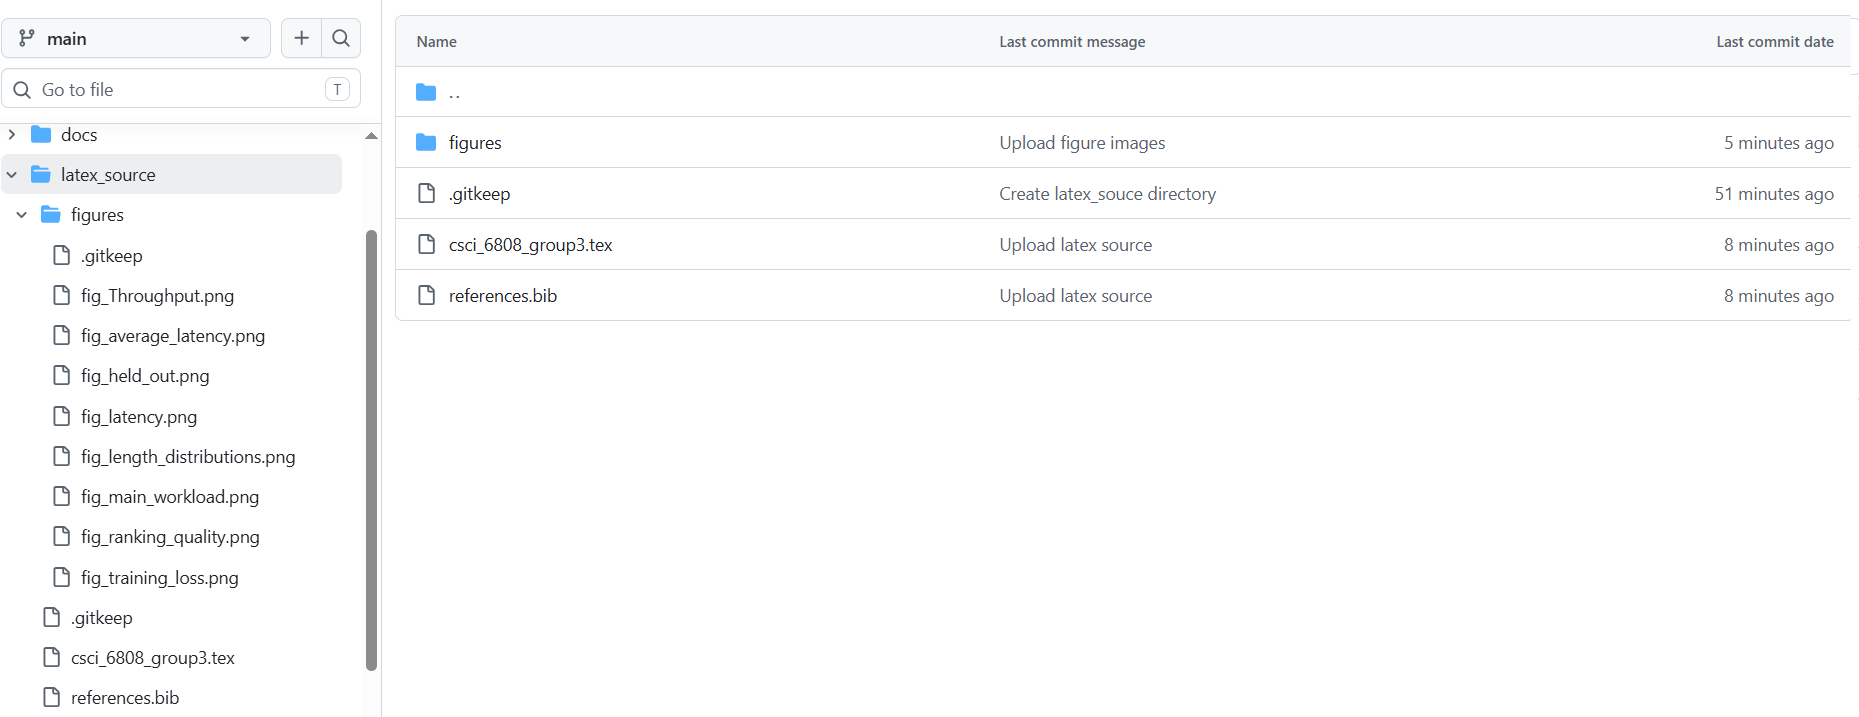
\includegraphics[width=0.95\linewidth]{figures/fig_app_folder.png}}
\caption{The \texttt{latex\_source} directory, pushed to the top level of the group's GitHub repository, showing the \texttt{figures/} subdirectory, the LaTeX source file, and \texttt{references.bib}.}
\label{fig:appendixghfolder}
\end{figure}

\clearpage
\bibliographystyle{IEEEtran}
\bibliography{references}

\end{document}
